%!TEX root = draft.tex
\section{Reducing Linearizability of Priority Queues to Reachability}
\label{sec:co-regular of extended priority queues}

We show that the set of executions for which some projection fails the test $\textit{Check-PQ-Conc-NonRec}$ can be characterized using a set of register automata, modulo a value renaming. The possibility of renaming values (which is complete for checking data independent implementations) allows to simplify the reasoning about projections. Thus, we assume that all the operations which are not in the projection failing this test use the same distinguished value $\top$, different from those used in the projection. Then, it is enough to find an automata characterization for the set of executions $e$ for which $\textit{Check-PQ-Conc-NonRec}$ fails, or equivalently, for which one
%a projection $e'$ fails $\textit{Check-PQ-Conc-NonRec}$ when one
of the following three formulas is false:
\begin{align*}
\hspace{-5mm}
\Gamma(e) := \mathsf{Has\text{-}}\Gamma(e) \Rightarrow \exists \alpha.\ \Gamma\mathsf{\text{-}Conc}(e,\alpha)\mbox{ with $\Gamma\in \{\mathsf{EmptyRemove}$, $\mathsf{UnmatchedMaxPriority}$, $\mathsf{MatchedMaxPriority}\}$}
\end{align*}
Intuitively, $\Gamma(e)$ states that $e$ is linearizable w.r.t. the set of sequential executions described by $\Gamma\mathsf{\text{-}Seq}$ (provided that $\mathsf{Has\text{-}}\Gamma(e)$ holds). Therefore, by an abuse of terminology, an execution $e$ satisfying $\Gamma(e)$ is called \emph{$\Gamma$-linearizable}.
Extending the automaton characterizing executions which are not $\Gamma$-linearizable, with self-loops that allow any operation with parameter $\top$ results in an automaton satisfying the following property called \emph{$\Gamma$-completeness}.

\begin{definition}
For $\Gamma\in \{\mathsf{EmptyRemove}$, $\mathsf{UnmatchedMaxPriority}$, $\mathsf{MatchedMaxPriority}\}$, an automaton $A$ is called \emph{$\Gamma$-complete} when for each data-independent implementation $\mathcal{I}$:

$A \cap \mathcal{I} \neq \emptyset$ if and only if there exists $ e \in \mathcal{I}$ and $e' \in \textit{proj}(e)$ such that $e'$ is not $\Gamma$-linearizable.
\end{definition}

The following result shows that deriving $\Gamma$-complete automata for each $\Gamma$ enables an effective reduction of checking linearizability of concurrent priority queue implementations to state reachability. It is a direct consequence of the above definitions.

\begin{restatable}{theorem}{ReduceEPQIntoStateReachability}
\label{lemma:reduce EPQ into state reachability}
Let $\mathcal{I}$ be a data-independent implementation, and $A(\Gamma)$ a $\Gamma$-complete automaton for each $\Gamma$. Then,
$\mathcal{I} \sqsubseteq \seqPQ$ if and only if $\mathcal{I} \cap A(\Gamma) = \emptyset$ for all $\Gamma$.
\end{restatable}

Section~\ref{ssec:aut} describes a $\mathsf{MatchedMaxPriority}$-complete automaton (TODO the other automata are discussed in Appendix~\ref{} or Icalp??) while Section~\ref{} discusses decidability results implied by the theorem above.

W.l.o.g., we assume that every implementation $\mathcal{I}$ behaves correctly, i.e., as a FIFO queue, when only values with the same priority are observed. More precisely, we assume that for every execution $e\in\mathcal{I}$ and every priority $p\in\mathbb{P}$, the projection of $e$ to values with priority $p$ is linearizable (w.r.t. $\seqPQ$). This property can be checked separately using the techniques introduced for regular FIFO queues in~\cite{DBLP:conf/icalp/BouajjaniEEH15} (see Appendix~\ref{} for more details). Note that this assumption excludes some obvious violations, such as a $\textit{rm}(a)$ operation happens before a $\textit{put}(a,p)$ operation, for some $p$.

Also, we consider $\Gamma$-complete automata for $\Gamma\in \{\mathsf{UnmatchedMaxPriority}, \mathsf{MatchedMaxPriority}\}$, recognizing executions which contains only one maximal priority. This is possible because any data-differentiated execution for which $\Gamma(e)$ is false has such a projection.
%Also, we consider $\Gamma$-complete automata for $\Gamma\in \{\mathsf{UnmatchedMaxPriority}, \mathsf{MatchedMaxPriority}\}$, recognizing executions where any two occurring priorities are comparable (w.r.t. $\prec$). This is possible because any data-differentiated execution which is not $\Gamma$-linearizable has such a projection.
Formally, given a data-differentiated execution $e$ and $p$ a maximal priority in $e$, $e\vert_{\preceq p}$ is the projection of $e$ to the set of values with priorities comparable to $p$. Then,

\begin{restatable}{lemma}{priExecutionIsEnough}
\label{lemma:pri execution is enough}
Let $\Gamma\in \{\mathsf{UnmatchedMaxPriority}, \mathsf{MatchedMaxPriority}\}$ and $e$ a data-differentiated execution. Then, $e$ is $\Gamma$-linearizable iff $e\vert_{\preceq p}$ is $\Gamma$-linearizable for some maximal priority $p$ in $e$.
\end{restatable}
\begin {proof} (Sketch)
%{\color {blue}We prove an equivalent property: $e$ is $\Gamma$-linearizable if and only if $e\vert_{\preceq p}$ is $\Gamma$-linearizable for some maximal priority $p$ in $e$.} %We consider the case of $\mathsf{MatchedMaxPriority}$ and the case of $\mathsf{UnmatchedMaxPriority}$ is similar.
To prove the $\textit{only if}$ direction, let $e$ be a data-differentiated execution linearizable w.r.t. $l = u \cdot \textit{put}(x,p) \cdot v \cdot \textit{rm}(x) \cdot w \in \mathsf{MatchedMaxPriority}\mathsf{\text{-}Seq}(s,x)$. Since $\mathsf{MatchedMaxPriority}\mathsf{\text{-}Seq}(s,x)$ imposes no restriction on the operations in $u$, $v$ and $w$ with priorities incomparable to $p$, erasing all these operations results in a sequential execution which still satisfies this property. Similarly, for $\Gamma=\mathsf{UnmatchedMaxPriority}$.

The $\textit{if}$ direction follows from the fact that if the projection of an execution to a set of operations $O_1$ has a linearization $l_1$ and the projection of the same execution to the remaining set of operations has a linearization $l_2$, then the execution has a linearization which is defined as an interleaving of $l_1$ and $l_2$ (see Appendix~\ref{} for more details).

Thus, let $e$ be an execution such that $e\vert_{\preceq p}$ is linearizable w.r.t. $l = u \cdot \textit{put}(x,p) \cdot v \cdot \textit{rm}(x) \cdot w \in \mathsf{MatchedMaxPriority}\mathsf{\text{-}Seq}(s,x)$. By the property above, we know that $e$ has a linearization $l' = u' \cdot \textit{put}(x,p) \cdot v' \cdot \textit{rm}(x) \cdot w'$, such that the projection of $l'$ to values of priority comparable to $p$ is $l$.
%We can see that $u$, $v$ and $w$ are subsequences of $u'$, $v'$ an $w'$, respectively.
Since $\mathsf{MatchedMaxPriority}\mathsf{\text{-}Seq}(s,x)$ does not have a condition on values of priority incomparable to $p$, we obtain that $l' \in \mathsf{MatchedMaxPriority}\mathsf{\text{-}Seq}(s,\alpha)$.
\end {proof}

%When the data domain and priority domain are both fixed to be finite set, the register automata can be simulated with finite automata, and by Lemma \ref{lemma:reduce EPQ into state reachability}, checking linearizable w.r.t $\seqPQ$ is decidable.


%
%
% and
%
%Let $A(\Gamma)$ be a $\Gamma$-complete automaton for each $\Gamma$. The following theorem
%
%
%We will describe this automaton only in the case of $\Gamma=\mathsf{MatchedMaxPriority}$. The rest can be found in Appendix~\ref{}. These automata satisfy the following property
%
%the main technical challenge is to show that each of the following sets of executions can be characterized in terms of automata (modulo renaming of values):
%
%
% define a set of register automata whose product with a given implementation $\mathcal{I}$ accepts a linearizability violation whenever $\mathcal{I}$ is not linearizable.
%
%are precise enough to recognize every non-linearizable implementation.
%
%In this section, we divide checking linearizability w.r.t $\seqPQ$ into checking linearizablity w.r.t $\Gamma\mathsf{\text{-}Seq}(s,\alpha)$, each of which can be done in polynomial-time. Due to data-independence, violations to each $\Gamma\mathsf{\text{-}Seq}(s,\alpha)$ can be captured by register automata. This reduces checking linearizability w.r.t $\seqPQ$ into state reachability problem.
%
%
%
%\subsection{Co-Regular}
%\label{subsec:definition of co-regular}
%



%Let $\Gamma\mathsf{\text{-}Condition}(e)$ be $\mathsf{HasEmptyRemoves}(e)$, $\neg \mathsf{HasEmptyRemoves}(e) \wedge \mathsf{HasUnmatchedMaxPriority}(e)$, and $\mathsf{HasMatchedMaxPriority}(e)$, for $\Gamma = \mathsf{EmptyRemove}, \mathsf{UnmatchedMaxPriority}, \mathsf{MatchedMaxPriority}$, respectively. $\textit{Check-PQ-Conc}$ inspires us that, when $\Gamma\mathsf{\text{-}Condition}(e)$ holds, there should exist some $\alpha$, such that  $\Gamma\mathsf{\text{-}Conc}(e,\alpha)$ holds. The following lemma states this formally. Let $\textit{proj}(e)$ be the set of projections of $e$ into set of values. When refer to $\textit{proj}(e)$, we implicitly assume that each $\textit{rm}(\textit{empty})$ in $e$ has a ghost argument that is unique. We say that execution $l$ is linearizable w.r.t $\Gamma$, if we can find a sequence $s$ where $e \sqsubseteq s$ and $\Gamma\mathsf{\text{-}Seq}(s,\alpha)$ holds for some $\alpha$.

%\begin{restatable}{lemma}{EPQasMultiInMRpriforHistory}
%\label{lemma:EPQ as multi in MRpri for history}
%Given a data-differentiated execution $e$, $e \sqsubseteq \seqPQ$, if and only if, $\forall e' \in \textit{proj}(e)$, $\forall \Gamma\in \{\mathsf{EmptyRemove}$, $\mathsf{UnmatchedMaxPriority}$ $,\mathsf{MatchedMaxPriority}\}$,  $\Gamma\mathsf{\text{-}Condition}(e)$ $\Rightarrow$ $e$ is linearizable w.r.t $\Gamma$.
%\end{restatable}


%Note that due to data-independence, register automata are used to detect some renamed violations, instead of store and checking directly. Let us introduce the notion of co-regular, which reduce checking linearizable w.r.t $\Gamma\mathsf{\text{-}Conc}(e,\alpha)$ into checking set of witness automata.
%
%%\vspace{-6pt}
%\begin{definition}\label{def:co-regular of rules of extended priority queues}
%Given $\Gamma\in \{\mathsf{EmptyRemove}$, $\mathsf{UnmatchedMaxPriority}$ $,\mathsf{MatchedMaxPriority}\}$. $\Gamma$ is co-regular, if there is a finite set $\textit{Auts}_{\Gamma}$ of register automata, such that for each data-independent implementation $\mathcal{I}$, we have that:
%
%$\textit{Auts}_{\Gamma} \cap \mathcal{I} \neq \emptyset$ if and only if $\exists e \in \mathcal{I}_{\neq},e' \in \textit{proj}(e)$, such that $\Gamma\mathsf{\text{-}Condition}(e')$ holds but $e$ does not linearizable w.r.t $\Gamma$.
%
%$\seqPQ$ is co-regular, if each $\Gamma$ is co-regular.
%\end{definition}

\subsection{A $\mathsf{MatchedMaxPriority}$-complete automaton}\label{ssec:aut}

%{\color {blue}When $\mathsf{MatchedMaxPriority}$ is false for some execution $e$, then there are two possibilities:
%
%\begin{itemize}
%\setlength{\itemsep}{0.5pt}
%\item[-] There exists value $x$, let $e_x$ be obtained from $e$ when all the values of maximal priorities in $e$ but $x$ are removed. Then $\mathsf{MatchedMaxPriority\text{-}Conc}(e_x,x)$ is false.
%
%\item[-] There exists set $X$ of values, let $e'$ be obtained from $e$ when all the values of maximal priorities in $e$ but values in $X$ are removed. Then, although $\mathsf{MatchedMaxPriority\text{-}Conc}(e'_x,x)$ is true for each $x \in X$, there is no value $y$ to make $\mathsf{MatchedMaxPriority\text{-}Conc}(e',y)$ to be true.
%\end{itemize}
%
%It is surprised to see that these two possibilities can be captured by two sub-cases of $\mathsf{MatchedMaxPriority}$, depending on whether is only one value $x$ with maximal priority $p$. We denote by $\mathsf{MatchedMaxPriority}^{>}$ the strengthening of $\mathsf{MatchedMaxPriority}$ with this condition (i.e., all the values other than $x$ have a priority strictly smaller than $p$) and $\mathsf{MatchedMaxPriority}^{=}$ for the strengthening of the same formula with the negation of this condition (i.e., there exists another value $y$ with priority $p$).
%}

A differentiated execution $e$ is not $\mathsf{MatchedMaxPriority}$-linearizable when all the $\textit{put}$ operations in $e$ using the maximal priority $p$ are matched, and $e$ is not linearizable w.r.t. the set of sequential executions satisfying $\mathsf{MatchedMaxPriority\text{-}Seq}(e,x)$ for each value $x$ of priority $p$. We consider two cases depending on whether $e$ contains exactly one value with priority $p$ or at least two values. We denote by $\mathsf{MatchedMaxPriority}^{>}$ the strengthening of $\mathsf{MatchedMaxPriority}$ with the condition that all the values other than $x$ have a priority strictly smaller than $p$ (corresponding to the first case), and by $\mathsf{MatchedMaxPriority}^{=}$ the strengthening of the same formula with the negation of this condition (corresponding to the second case).
We use particular instances of register automata~\cite{finite-memory, the paper I found} whose states include only two registers, one for storing a priority guessed at the initial state, and one for storing the priority of the current action in the execution. The transitions can check equality or the order relation $\prec$ between the values stored in the two registers. Instead of formalizing the full class of register automata, we consider a simpler class which suffices our needs. More precisely, we consider a class of labeled transition systems whose states consist of a finite control part and a register $r$ interpreted to elements of $\mathbb{P}$. The transition labels can be one of the following:
\begin{itemize}
	\item $r=*$ for storing an arbitrary value to $r$,
	\item $\textit{call}(\textit{rm},a)$ and $\textit{ret}(\textit{rm},a)$ for reading call/return actions of a remove,
	\item $\textit{call}(\textit{put},d,g)$ where $g\in\{=r,\prec r,true\}$ is a guard, for reading a call action $\textit{call}(\textit{put},d,p)$ of a put and checking whether $p$ is either equal to or smaller than the value stored in $r$, or arbitrary,
	\item $\textit{ret}(\textit{put},d,true)$ for reading a return action $\textit{ret}(\textit{put},d,p)$ for some $p$.
\end{itemize}
The set of words accepted by such a transition system can be defined as usual.

%$\textit{call}(\textit{put},d,g)$ $\textit{ret}(\textit{put},d,g),$ $\textit{call}(\textit{rm},d),\textit{ret}(\textit{rm},d)$, where $d \in \mathbb{D} \cup \{ \textit{empty} \}$, and $g$ and $\top$ are guards
%
% which are complete for each case. Since we don't require the full generality of register automata,
%
%
%We define $\Gamma$-complete automata for both cases and their union will give a $\mathsf{MatchedMaxPriority}$-complete automaton
%
%
%
%Register automata is a kind of finite automata with registers used to deal with infinite data domain, where register can be assigned values and do simple operations. In this paper we use a restricted kind of register automata, which contains only one register, whose value is obtained once by guessing and never changed. Our register machine contains a register $r$. Its transition labels are $r=*,\textit{call}(\textit{put},d,g), \textit{ret}(\textit{put},d,g),$ $\textit{call}(\textit{rm},d),\textit{ret}(\textit{rm},d)$, where $d \in \mathbb{D} \cup \{ \textit{empty} \}$, and $g$ and $\top$ are guards. The first transition from initial state is a $r=*$ transition, and is used to assign an arbitrary value to $r$. A guard is a predicate chosen from $\{=r,< r,\top \}$, which represents equals the value of $r$, less than the value of $r$, and always holds, respectively. Given an execution $e = \alpha_1 \cdots \alpha_k$ of priority queue, register automata $\mathcal{A}$ accepts $e$, if there exists value $d_r\in \mathbb{D}$ and transitions $q_0 \xrightarrow{\beta_1} q_1 \ldots \xrightarrow{\beta_k} q_k$ of $\mathcal{A}$ from a initial state to a final state, such that for each $i$
%
%\begin{itemize}
%\setlength{\itemsep}{0.5pt}
%\item[-] If $\alpha_i = \textit{call}(\textit{put},a,p)$, then $\beta_i= \textit{call}(\textit{put},a,g)$ and $g$ holds with $p$ and $d_r$. Similarly for $\textit{ret}(\textit{put},a,p)$.
%
%\item[-] Else, $\alpha_i = \beta_i$.
%\end{itemize}


\subsubsection{A $\mathsf{MatchedMaxPriority}^>$-complete automaton}
\label{subsec:co-regular of EPQ1Lar}


%We use two point to simply our proof of co-regular. The first point is to use the results in \cite{Bouajjani:2015} to ensure FIFO (first in first out) property of each single-priority projections. A execution where only values of one priority is putted is called a single-priority execution. It is obvious that each single-priority projection of sequences in $\seqPQ$ satisfy FIFO property. Let $\textit{toQueue}(e)$ be an execution generated from $e$ by transforming $\textit{put}$ and $\textit{rm}$ into $\textit{enq}$ and $\textit{deq}$, respectively, and then discarding priorities. In Appendix \ref{sec:appendix proof and definition in section definition of co-regular}, according to the result of queue in \cite{Bouajjani:2015}, we construct a set $\textit{Auts}_{\textit{sinPri}}$ of witness automata, and shows that they are enough to ensure that for each data-differentiated executions, each of its single-priority projection without $\textit{rm}(\textit{empty})$ to have ``FIFO'' property, as shown by the following lemma.
%
%\begin{restatable}{lemma}{AutoForEPQwithSignlePri}
%\label{lemma:automata for extended priority queue with single priority}
%
%Given a data-independent implementations $\mathcal{I}$ of extended priority queue, $\mathcal{I} \cap \textit{Auts}_{\textit{sinPri}} \neq \emptyset$, if and only if there exists $e \in \mathcal{I}_{\neq}$, $e' \in \textit{proj}(e)$, such that $e'$ is single-priority  without $\textit{rm}(\textit{empty})$, and $\textit{toQueue}(e')$ does not linearizable to queue.
%\end{restatable}
%
%According to Lemma \ref{lemma:automata for extended priority queue with single priority}, from now on, it is safe to assume that, for each data-differentiated execution, any of its single-priority projection without $\textit{rm}(\textit{empty})$ has ``FIFO'' property. This effectively exclude some obvious violations, such as $\textit{rm}(a)$ happens before $\textit{put}(a,\_)$.


%Lemma \ref{lemma:pri execution is enough} makes our co-regular proof more clear. One consequence of it is that for given $e\vert_{\preceq p}$, $\Gamma\mathsf{\text{-}Condition}(e')$ holds only for one $\Gamma$.
%
%
%
%
%
%
%\subsection{Co-Regular of $\mathsf{MatchedMaxPriority}^{>}$}
%\label{subsec:co-regular of EPQ1Lar}

%To facilitate the proof of co-Regular of $\mathsf{MatchedMaxPriority}$, we separate $\mathsf{MatchedMaxPriority\text{-}Seq}(e,x)$ into the following two sub-predicates, where the first one represents that $x$ is the only value with priority $p$ in $e$ , and the second one represents that there are more than one value with priority $p$ in $e$. Here $\textit{occurOnce}(p,l)$ holds if there is only one value with priority $p$ in $l$.
%
%{\small
%\begin{align*}
%\mathsf{MatchedMaxPriority}^{>}\mathsf{\text{-}Seq}(e,x)=\mathsf{true} & \mbox{ iff  $\mathsf{MatchedMaxPriority}\mathsf{\text{-}Seq}(e,x)=\mathsf{true}$,} \\
%&\hspace{4mm}\mbox{$\textit{occurOnce}(p,e)$ where $p$ is the priority of $x$} \\
%\mathsf{MatchedMaxPriority}^{=}\mathsf{\text{-}Seq}(e,x)=\mathsf{true} & \mbox{ iff  $\mathsf{MatchedMaxPriority}\mathsf{\text{-}Seq}(e,x)=\mathsf{true}$,} \\
%&\hspace{4mm}\mbox{$\neg\textit{occurOnce}(p,e)$ where $p$ is the priority of $x$} \\
%\end{align*}
%}
%
%$\mathsf{MatchedMaxPriority}^{>}\mathsf{\text{-}Conc}(e,x)$ is obtained from $\mathsf{MatchedMaxPriority}\mathsf{\text{-}Conc}(e,x)$ by using $\mathsf{MatchedMaxPriority}^{>}\mathsf{\text{-}Seq}(e,x)$ instead of $\mathsf{MatchedMaxPriority\text{-}Seq}(e,x)$. And similarly for $\mathsf{MatchedMaxPriority}^{=}\mathsf{\text{-}Conc}(e,x)$.
%
%We can also define two conditions, where $\textit{unmatched-priorities}(l)$ is the set of priorities occurring in $\textit{put}$ operations of $e$ for which there is $\textit{rm}$ operation removing the same value:
%
%{\small
%\begin{align*}
%\mathsf{MatchedMaxPriority}^{>}\mathsf{\text{-}Condition}(e)=\mathsf{true} & \mbox{ iff $p\in \textit{matched-priorities}(e)$ for a maximal priority} \\
%&\hspace{4mm}\mbox{$p\in priorities(e)$, $\textit{occurOnce}(p,e)$} \\
%\mathsf{MatchedMaxPriority}^{=}\mathsf{\text{-}Condition}(e)=\mathsf{true} & \mbox{ iff $p\in \textit{matched-priorities}(e)$ for a maximal priority} \\
%&\hspace{4mm}\mbox{$p\in priorities(e)$, $\neg\textit{occurOnce}(p,e)$}
%\end{align*}}
We give a typical example of an execution $e$ which is not $\mathsf{MatchedMaxPriority}^>$-linearizable in
%Given a data-differentiated execution $e$ such that $\mathsf{MatchedMaxPriority}^{>}\mathsf{\text{-}Condition}(e)$ holds, Lemma \ref{lemma:automata for extended priority queue with single priority} is not enough for ensure linearizable w.r.t $\mathsf{MatchedMaxPriority}^{>}$. This is because that it is possible that $\mathsf{MatchedMaxPriority}^{>}\mathsf{\text{-}Conc}(e,x)$ does not holds because of interaction between actions of multiple priorities. One such example is shown in
\figurename~\ref{fig:introduce gap for EPQ1Lar}. Intuitively, this is a violation because during the whole execution of $\textit{rm}(b)$, the priority queue stores a smaller priority value (which should be removed before $b$). To be more precise, we define \emph{the interval of a value $x$} as the time interval from the return of a put $\textit{ret}(\textit{put},x,p)$ to the call of the matching remove $\textit{call}(rm,x)$, or to the end of the execution if such a call action doesn't exist. Intuitively, it represents the time interval in which a value is guaranteed to be stored into the concurrent priority queue.
In \figurename~\ref{fig:introduce gap for EPQ1Lar}, we draw the interval of each value by dashed line. Here we assume that $p_1 \prec p_4$, $p_2 \prec p_4$, and $p_3 \prec p_4$. We can not find a sequence $s$ where $e \sqsubseteq s$ and $\mathsf{MatchedMaxPriority}\mathsf{\text{-}Seq}(s,b)$ holds, since each time point from $\textit{call}(\textit{rm},b)$ to $\textit{ret}(\textit{rm},b)$ is included in the interval of some smaller priority value, and $\textit{rm}(b)$ can't take effect in the interval of a smaller priority value.

\begin{figure}[htbp]
  \centering
  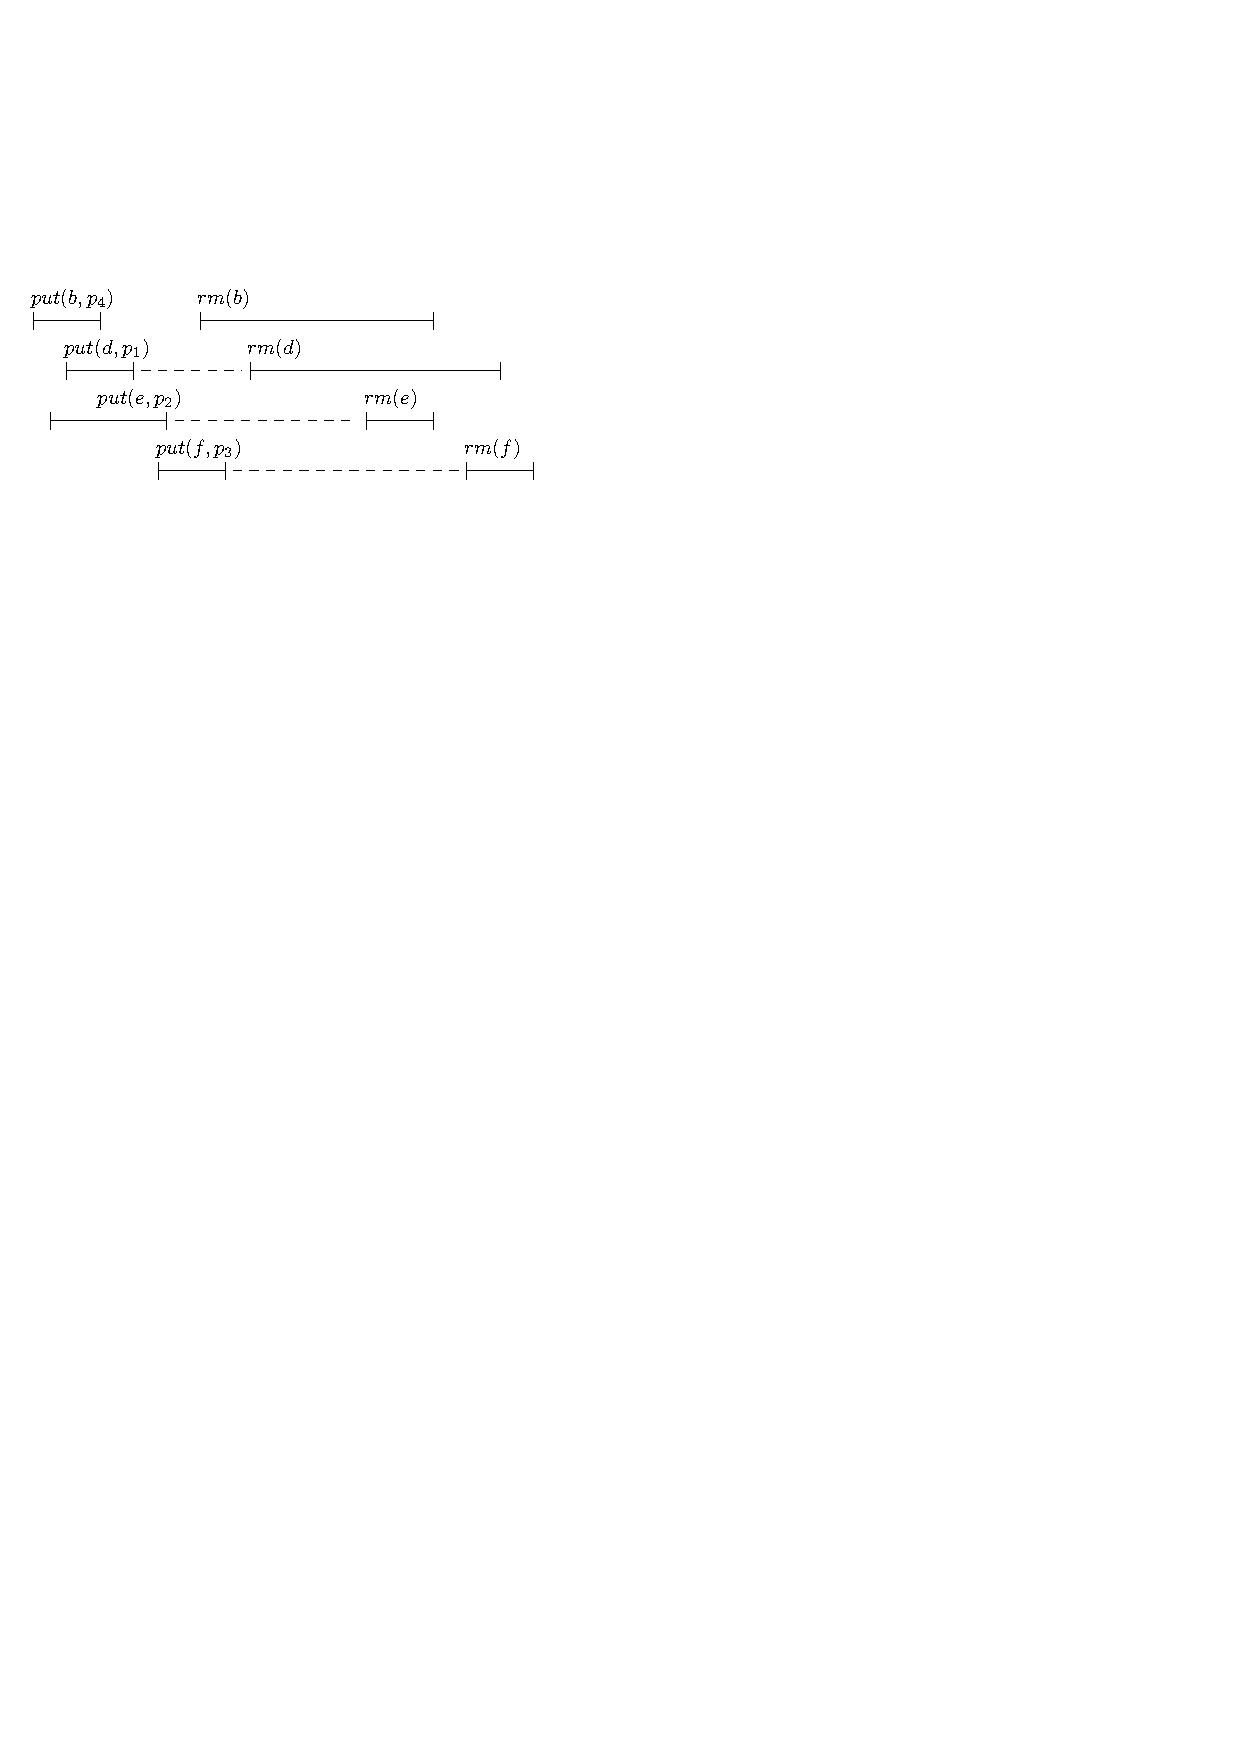
\includegraphics[width=0.4 \textwidth]{figures/PIC-HIS-INTRO-GAP-EPQ1L.pdf}
%\vspace{-10pt}
  \caption{An execution that is not $\mathsf{MatchedMaxPriority}^{>}$-linearizable}
  \label{fig:introduce gap for EPQ1Lar}
\end{figure}

To formalize the scenario in \figurename~\ref{fig:introduce gap for EPQ1Lar} we use the notion of \emph{left-right constraint} defined below.

\begin{definition}\label{def:left-right constraint for matched put and rm operations}
Let $e$ be a data-differentiated execution which contains only one maximal priority $p$, and only one value $x$ of priority $p$ (and no $\textit{rm}(\textit{empty})$ operations).
% and let $\textit{put}(x,p)$ and $\textit{rm}(x)$ be the only operations with priority $p$.
The \emph{left-right constraint of $x$} is the graph $G$ where: %$\textit{put}(x,p)$ and $\textit{rm}(x)$ is the graph $G$ where:
\begin{itemize}
\item the nodes are the values occurring in $e$, %, to which we add a node,
\item there is an edge from $d_1$ to $x$, if $\textit{put}(d_1,\_) <_{\textit{hb}} \textit{put}(x,p)$ or $\textit{put}(d_1,\_) <_{\textit{hb}} \textit{rm}(x)$,
\item there is an edge from $x$ to $d_1$, if $\textit{rm}(x)<_{\textit{hb}}\textit{rm}(d_1)$ or $\textit{rm}(d_1)$ does not exists,
\item there is an edge from $d_1$ to $d_2$, if $\textit{put}(d_1,\_) <_{\textit{hb}} \textit{rm}(d_2,\_)$.
\end{itemize}
\end{definition}

The execution in \figurename~\ref{fig:introduce gap for EPQ1Lar} is not $\mathsf{MatchedMaxPriority}^>$-linearizable because the left-right constraint of the maximal priority value $b$ contains a cycle: $f \rightarrow e \rightarrow d \rightarrow b \rightarrow f$. We prove that the presence of such a cycle is equivalent to the execution not being $\mathsf{MatchedMaxPriority}^>$-linearizable (see Appendix~\ref{}).
%The existence of cycle though value with maximal priority in left-right constraint formally modelled the phenomenon in \figurename~\ref{fig:introduce gap for EPQ1Lar}. For example, in \figurename~\ref{fig:introduce gap for EPQ1Lar}, $f \rightarrow e \rightarrow d \rightarrow b \rightarrow f$ is a cycle in left-right constraint. We then prove that getting rid of cycle though value with maximal priority in left-right constraint is enough for ensure linearizable w.r.t $\mathsf{MatchedMaxPriority}^{>}$.
When the left-right constraint of the maximal priority value $x$ contains a cycle of the form $d_1 \rightarrow \ldots \rightarrow d_m \rightarrow x \rightarrow d_1$ for some $d_1$,$\ldots$,$d_n\in \mathbb{D}$, we say that $x$ is \emph{covered} by $d_1,\ldots,d_m$. The shape of such a cycle can be detected using our class of automata, the only complication being the unbounded number of values $d_1$,$\ldots$,$d_n$. However, by data independence, whenever an implementation contains such an execution it also contains an execution where all the values $d_1$,$\ldots$,$d_n$ are renamed to the same value $a$, and $x$ is renamed to $b$. Therefore, our automata can be defined over a fixed set of values $a$, $b$, and $\top$ (for the operations outside of the non-linearizable projection).

TODO WHY IT IS A SET OF AUTOMATA ? SAY WHAT ARE THE CASES THAT NEED TO BE COVERED. SAY WHAT IS THE CASE WE GIVE IN THE FIGURE. USE $\top$ AS MENTIONED AT THE BEGINNING OF THE SECTION INSTEAD OF 	$c$. USE BIG CAPS FOR SETS OF TRANSITION LABELS.

{\color {blue} Assume that $x$ is covered by $d_1,\ldots,d_m$, we can safely rename $x$ into $b$, rename $d_1,\ldots,d_m$ into $a$ and rename all other value into $c$ by data-independence. Since there are four cases of projection of execution to $x$ when their is a cycle through $x$. To ease the reading, for each of such case we generate a register automata, and then let the $\mathsf{MatchedMaxPriority}^{>}$-complete automaton be the union of the four register automata. For example, for the case when the projection of $e$ to $x$ is as in \figurename~\ref{fig:introduce gap for EPQ1Lar} (rename $b$ into $x$), we construct a register automaton $\mathcal{A}_{\textit{l-lar}}^1$ in \figurename~\ref{fig:automata APQ1Lar-1 in paper}. Here transition labels $c_1 = c + \textit{ret}(\textit{rm},a)$, $c_2 = c + \textit{call}(\textit{put},a,=r)$, $c_3 = c_2 + \textit{ret}(\textit{rm},a)$, where $c = \textit{call}(\textit{put},\top,\textit{true}),\textit{ret}(\textit{put},\top,\textit{true}), \textit{call}(\textit{rm},d)$, $\textit{ret}(\textit{rm},d),\textit{call}(\textit{rm},\textit{empty}),\textit{ret}(\textit{rm},\textit{empty})$. There are three paths in \figurename~\ref{fig:introduce gap for EPQ1Lar} from $q_{\textit{init}}$ to $q_7$, and they comes from that there are three possible positions for the first $\textit{call}(\textit{put},a,\_)$ in the captured execution, which is shown in \figurename~\ref{fig:executions APQ1Lar-1 in paper}. In \figurename~\ref{fig:automata APQ1Lar-1 in paper}, the paths $q_1 \rightarrow q_2 \rightarrow q_3 \ldots \rightarrow q_7$, $q_1 \rightarrow q_2 \rightarrow q_3 \ldots \rightarrow q_{10}$ and $q_1 \rightarrow q_9 \rightarrow q_{10} \ldots \rightarrow q_7$ corresponds to the first, second and third cases in \figurename~\ref{fig:executions APQ1Lar-1 in paper}, respectively.
}

\begin{figure}[htbp]
  \centering
  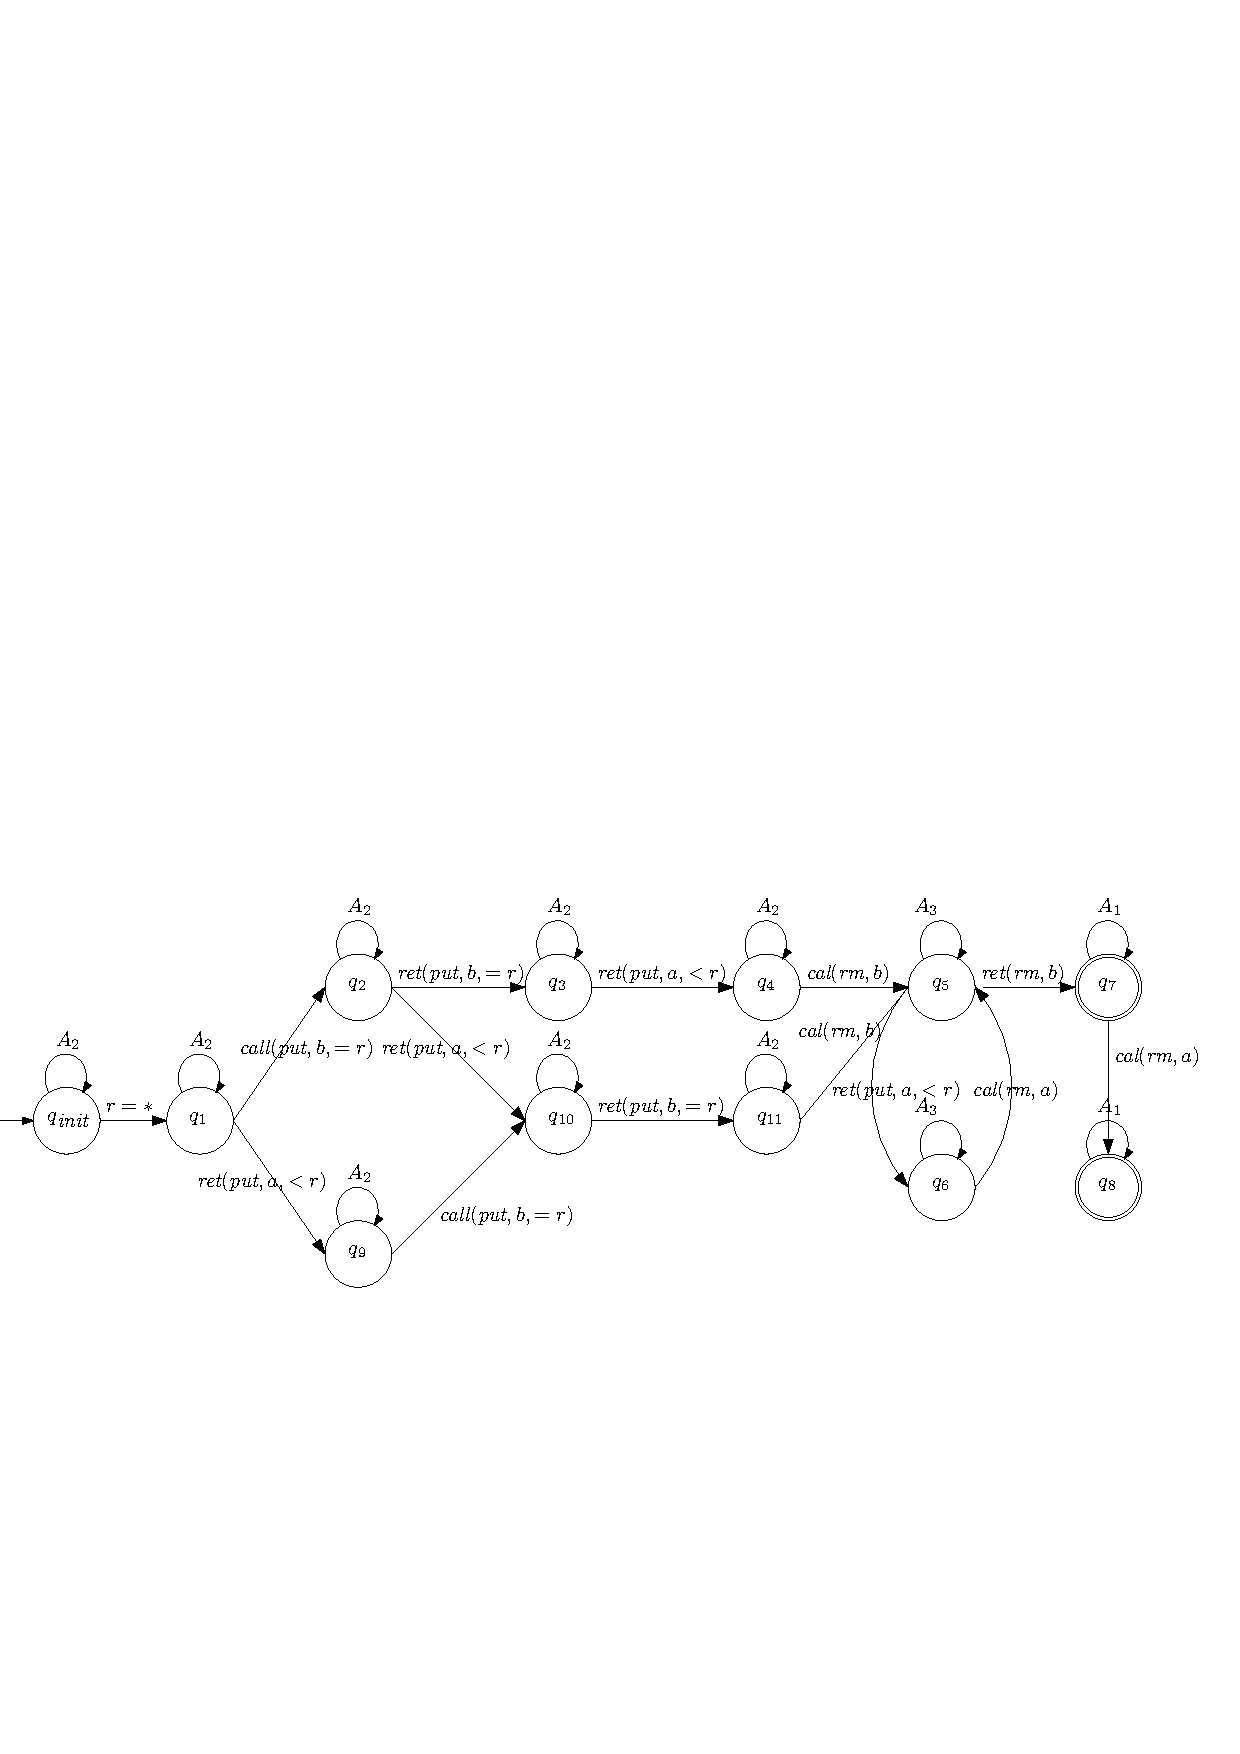
\includegraphics[width=1 \textwidth]{figures/PIC_AUTO_PQ1Lar-pprr.pdf}
%\vspace{-10pt}
  \caption{Automaton $\mathcal{A}_{\textit{l-lar}}^1$}
  \label{fig:automata APQ1Lar-1 in paper}
\end{figure}

\begin{figure}[htbp]
  \centering
  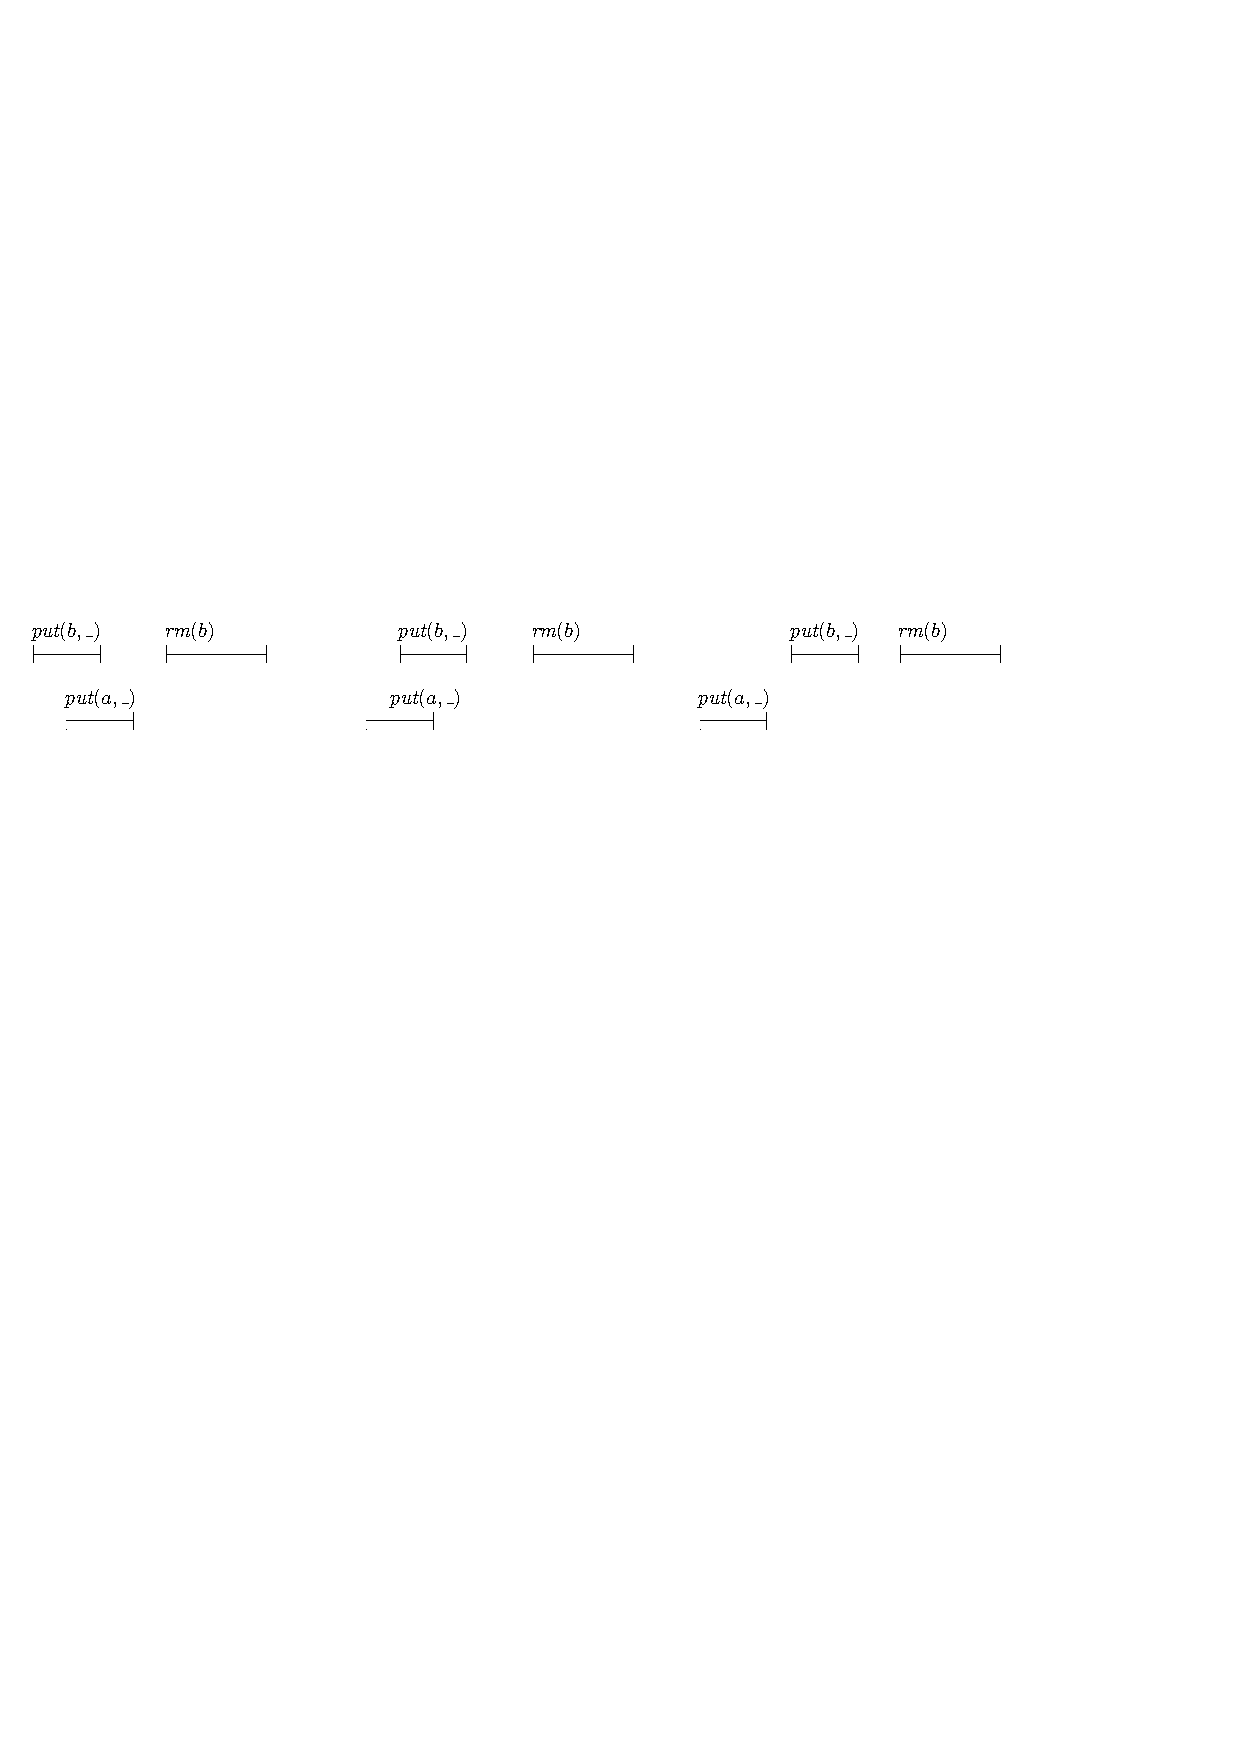
\includegraphics[width=1 \textwidth]{figures/PIC_HIS_PQ1Lar-pprr-in-paper.pdf}
%\vspace{-10pt}
  \caption{Three possible positions of the first $\textit{call}(\textit{put},a,\_)$ in captured execution}
  \label{fig:executions APQ1Lar-1 in paper}
\end{figure}


{\color {blue}
Let $\mathcal{A}_{\textit{1-lar}}$ be the union of the four register automata mentioned above, then we prove that $\mathcal{A}_{\textit{1-lar}}$ is $\mathsf{MatchedMaxPriority}^{>}$-complete. The detailed construction and proof can be found in Appendix \ref{sec:appendix proof and definition in section co-regular of EPQ1Lar}.
}

\begin{restatable}{lemma}{EPQOneLarisCoRegular}
\label{lemma:EPQ1Lar is co-regular}
$\textit{Auts}_{\textit{1-lar}}$ is $\mathsf{MatchedMaxPriority}^{>}$-complete.
\end{restatable}


More details can be found in Appendix \ref{sec:appendix proof and definition in section co-regular of EPQ1Lar}. %TODO MOVE THIS TO THE RELATED WORK


\subsubsection{A $\mathsf{MatchedMaxPriority}^=$-complete automaton}
\label{subsec:co-regular of EPQ1Equal}

In this subsection, we briefly introduce the idea for proving co-regular of $\mathsf{MatchedMaxPriority}^{=}$. The proof of this subsection can be found in Appendix \ref{sec:appendix proof and definition in section co-regular of EPQ1Equal}.

Given a data-differentiated $\_$-execution $e$ such that $\mathsf{MatchedMaxPriority}^{=}\mathsf{\text{-}Condition}(e)$ holds, Lemma \ref{lemma:automata for extended priority queue with single priority} and $\textit{Auts}_{\textit{1-lar}}$ are sill not enough for ensure that $e$ linearizable w.r.t $\mathsf{MatchedMaxPriority}^{=}$. This is because that given values $a$ and $b$ with maximal priority, it is possible that all the possible linearization points of $\textit{rm}(b)$ are disabled by $\textit{rm}(b)$. We give an example of such execution $e$ in \figurename~\ref{fig:introduce pb order}. The execution $e$ of \figurename~\ref{fig:introduce pb order} is not linearizable w.r.t $\mathsf{MatchedMaxPriority}^{=}$, even if $h \vert_{p_1}$ and $h \vert_{p_4}$ both linearizable w.r.t $\mathsf{MatchedMaxPriority}^{>}$, and either $a$ or $b$ is covered by values with smaller priority. The explanation of $e$ not linearizable w.r.t $\mathsf{MatchedMaxPriority}^{=}$ is as follows: Since $\textit{put}(a,p_4) <_{\textit{hb}} \textit{put}(b,p_4)$, the linearization points of $\textit{rm}(a)$ should before the linearization point of $\textit{rm}(b)$. According to the previous section, which says that linearizaton point of larger priority can be happen in the interval of values with smaller priority. Thus, the time intervals identified with dotted lines in \figurename~\ref{fig:introduce pb order} are are possible position to locate the linearization point of $\textit{rm}(b)$. However, each of them is before $\textit{call}(\textit{rm},a)$.

\begin{figure}[htbp]
  \centering
  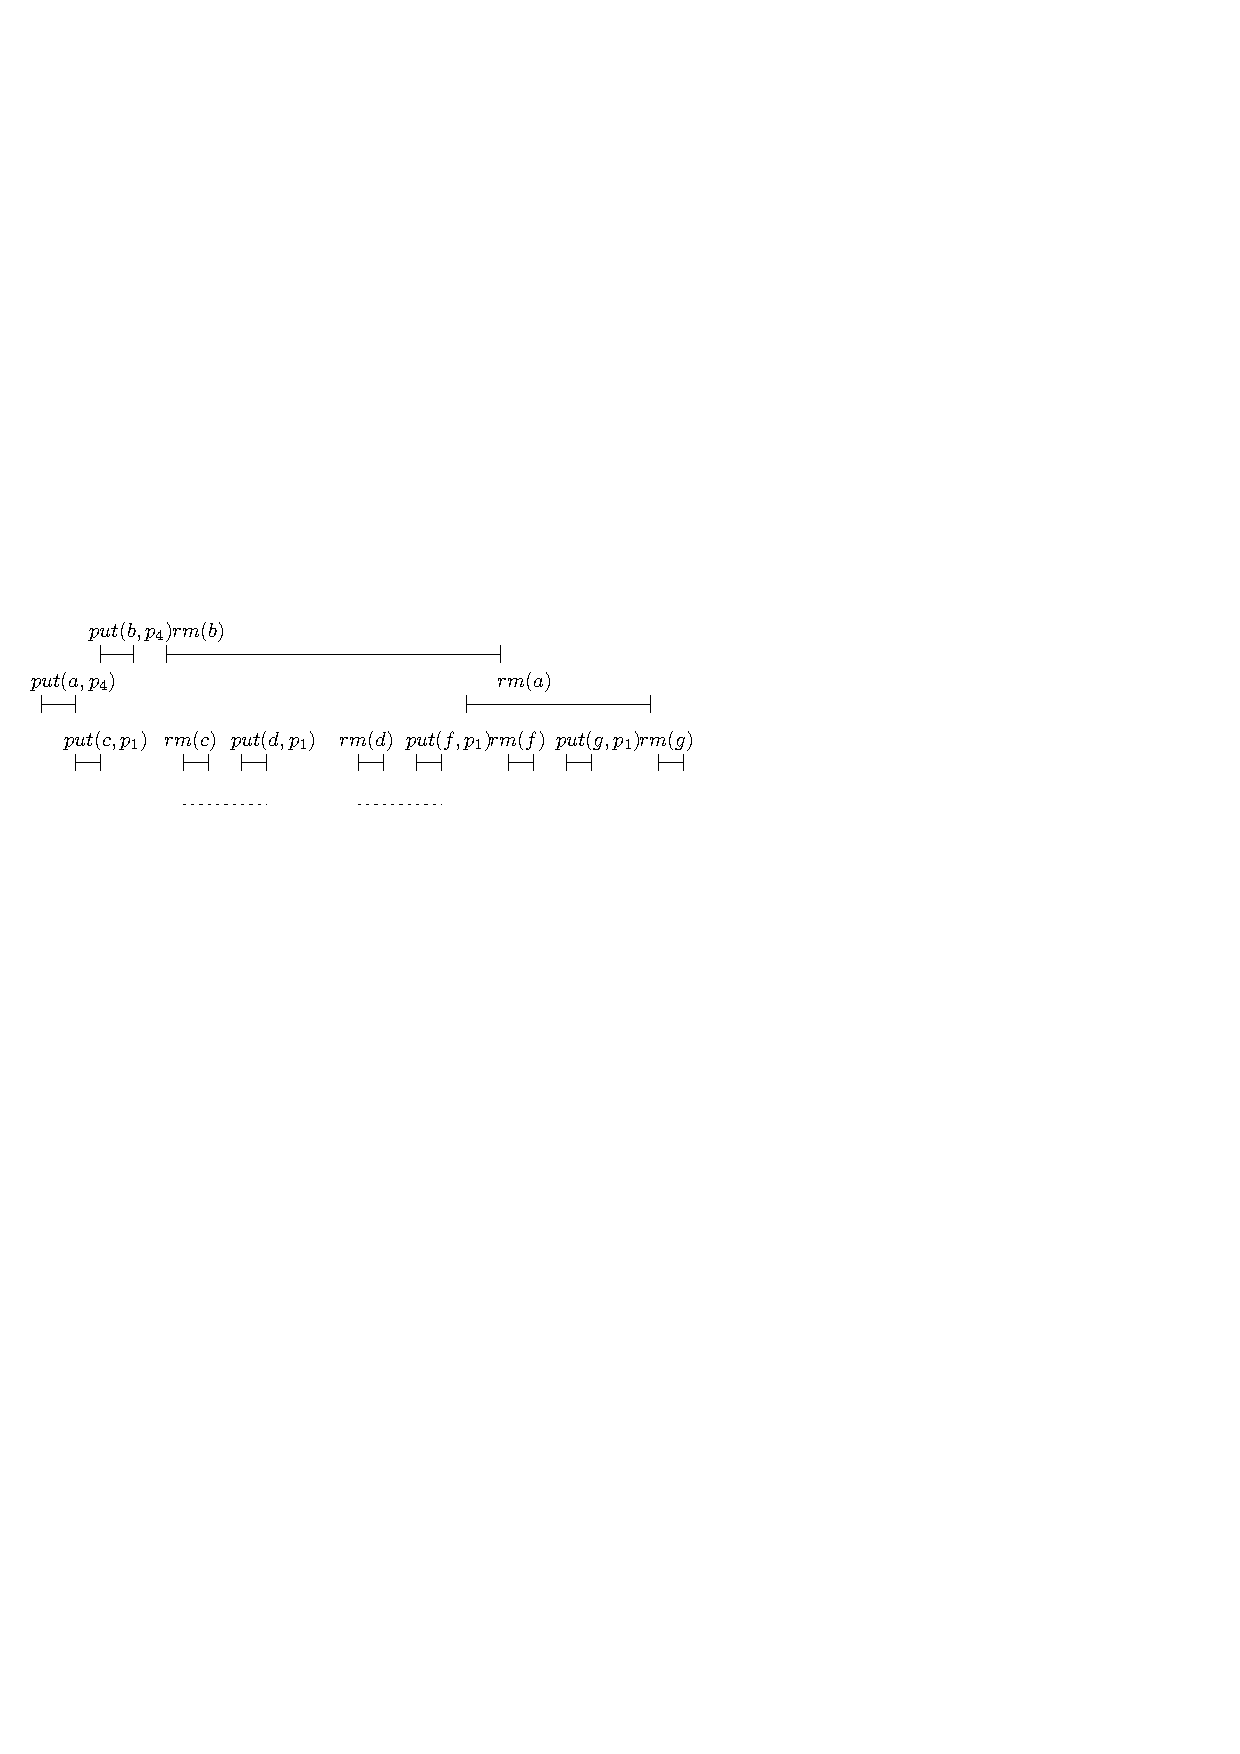
\includegraphics[width=0.6 \textwidth]{figures/PIC-HIS-INTRO-PB-ORDER-EPQ.pdf}
%\vspace{-10pt}
  \caption{An execution that does not linearizable w.r.t $\textit{MS}(\textit{EPQ}_1^{=})$}
  \label{fig:introduce pb order}
\end{figure}

One point need to be modeled in \figurename~\ref{fig:introduce pb order} is that ``a is putted before b''. Let us introduce put-before order $<_{\textit{pb}}$ to formally state that ``an value is putted before another value''. Given a data-differentiated $\_$-execution $e$ and two values $a,b$ with maximal priority, $a <_{\textit{pb}} b$, if one of the following cases holds: (1) $\textit{put}(a,\_) <_{\textit{hb}} \textit{put}(b,\_)$, (2) $\textit{rm}(a) <_{\textit{hb}} \textit{rm}(b)$, or (3) $\textit{rm}(a) <_{\textit{hb}} \textit{put}(b,\_)$. Sometimes we use $a <_{\textit{pb}}^A b$, $a <_{\textit{pb}}^B b$ and $a <_{\textit{pb}}^C b$ to explicitly distinguish above three cases. Let $<_{\textit{pb}}^*$ be the transitive closure of $<_{\textit{pb}}$. Intuitively, $a <_{\textit{pb}}^* b$ means that we can infer that $a$ is putted before $b$ with the help of several intermediate values.

Another point need to be modeled in \figurename~\ref{fig:introduce pb order} is the possible time points of $\textit{rm}(b)$, which is formally modeled by gap-point.

\begin{definition}\label{def:gap-point for matched put and rm operations}
Given a data-differentiated $p$-execution $e$ and two method events $\textit{put}(x,p),\textit{rm}(x)$ of $e$. We say that a time-point $o$ is a gap-point of $x$, if $o$ is after $\textit{call}(\textit{put},x,p)$ and $\textit{call}(\textit{rm},x)$, is before $\textit{ret}(\textit{rm},x)$, and is not in interval of any values with smaller priority.
\end{definition}

The case of \figurename~\ref{fig:introduce pb order} can be formally described as follows: $a <_{\textit{pb}}^* b$, while the right-most gap-point of $b$ is before $\textit{call}(\textit{rm},a)$ or $\textit{call}(\textit{put},a,p_4)$. The following lemma states that getting rid of such case is enough for ensure linearizable w.r.t $\mathsf{MatchedMaxPriority}^{=}$.

\begin{restatable}{lemma}{EPQOneEqualAsPBandGP}
\label{lemma:EPQ1Equal as pb order and gap-point}
Given a data-differentiated $p$-execution $e$ where $\mathsf{MatchedMaxPriority}^{=}\mathsf{\text{-}Condition}(e)$ holds. $e$ is not linearizable w.r.t $\mathsf{MatchedMaxPriority}^{=}$, if and only if there exists $x$ and $y$ with maximal priority $p$, such that $y <_{\textit{pb}}^* x$, and the rightmost gap-point of $x$ is before $\textit{call}(\textit{put},y,p)$ or $\textit{call}(\textit{rm},y)$ in $e$.
\end{restatable}

\begin {proof} (Sketch)

We have already intuitively explain the proof of the $\textit{if}$ direction. To prove the $\textit{only if}$ direction, we prove its contrapositive. %, where we already know that $\forall x, y$ with maximal priority, if $y <_{\textit{pb}}^* x$, then the rightmost gap-point of $x$ is after $\textit{cal}(\textit{put},y,\textit{pri})$ and $\textit{cal}(\textit{rm},x)$. We need to prove that $e \sqsubseteq \textit{MS}(\textit{EPQ}_1^{=})$. %Or we can say, we need to explicitly construct linearization of $e$.

Let $\textit{Items}(e,p)$ be the set of values with priority $p$ in $e$. We introduce another lemma (Lemma \ref{lemma:maximal in pb and gap-point make a candidate of EPQ1Equal} in Appendix), which states that if we can find a value $\exists g_1 \in \textit{Items}(e,p)$, such that $\forall g_2 \in \textit{Items}(e,p)$, (1) $g_1 \nless_{\textit{pb}} g_2$, and (2) the right-most gap-point of $g_1$ is after $\textit{call}(\textit{put},g_2,p)$ and $\textit{call}(\textit{rm},g_2)$. Then $e$ is linearizable w.r.t $\mathsf{MatchedMaxPriority}^{=}$.
The remaining of our proof is a loop for searching such $g_1$ in $e$. Let $e_p$ be the projection of $e$ into values of priority $p$, and let $l_p$ be the linearization of $e$ which satisfy the requirements of queue. Let the initial value of $a_1$ be the last inserted value in $l_p$.

\begin{itemize}
\setlength{\itemsep}{0.5pt}
\item[-] check if $a_1$ satisfy the conditions of Lemma \ref{lemma:maximal in pb and gap-point make a candidate of EPQ1Equal}. If it does, then this loop terminates.

\item[-] Otherwise, $\exists a_2 \in \textit{Items}(e,p)$, such that the rightmost gap-point of $a_1$ is before $\textit{cal}(\textit{put},a_2,p)$ or $\textit{cal}(\textit{rm},a_2)$ in $e$. By assumption, we know that $a_2 \nless_{\textit{pb}} a_1$, and each gap-point of $a_2$ is after the rightmost gap-point of $a_1$.

    \begin{itemize}
    \setlength{\itemsep}{0.5pt}
    \item[-] If $\forall b \in \textit{Items}(e,p)$, $a_2\not<_{\textit{pb}}b$. Then we go to next round of the loop and make $a_2$ to be the ``new-round $a_1$''.
    \item[-] Otherwise, there exists $a_3 \in \textit{Items}(e,p)$ such that $a_2 <_{\textit{pb}}^* a_3$. It is not hard to see that there is no cycle in $<_{\textit{pb}}$, and it is safe to assume that $a_3$ is maximal w.r.t $<_{\textit{pb}}^*$.

        By assumption,we know that the rightmost gap-point of $a_3$ is after $\textit{call}(\textit{put},a_2,p)$ and $\textit{call}(\textit{rm},a_2)$. Therefore, we can see that the rightmost gap-point of $a_3$ is after the rightmost gap-point of $a_1$. Then we go to next round of the loop and make $a_3$ to be the ``new-round $a_1$''.
    \end{itemize}
\end{itemize}

Let $a^i$ be the $a_1$ in the $\textit{i-th}$ round of loop. We can see that the rightmost gap-point of $a^j$ is after the rightmost gap-point of $a^i$ for each $i<j$. Therefore, the loop finally terminates at some $a^f$ that satisfies the condition of Lemma \ref{lemma:maximal in pb and gap-point make a candidate of EPQ1Equal}. This implies that $e$ is linearizable w.r.t $\mathsf{MatchedMaxPriority}^{=}$ and completes the proof of the $\textit{only if}$ direction. \qed
\end {proof}

The result of Lemma \ref{lemma:EPQ1Equal as pb order and gap-point} still needs to be impove, since obtaining $y <_{\textit{pb}}^* x$ may requires arbitrary many intermediate values, and it is hard to store unbounded values by automata. Fortunately, we prove that the number of intermediate values is essentially bounded, as stated by the following lemma.

\begin{restatable}{lemma}{OBOrderHasBoundedLength}
\label{lemma:ob order has bounded length}
Given a data-differentiated execution $e$. Assume that $a <_{\textit{pb}} a_1 <_{\textit{pb}} \ldots <_{\textit{pb}} a_m <_{\textit{pb}} b$, then one of the following cases holds:

\begin{itemize}
\setlength{\itemsep}{0.5pt}
\item[-] $a <_{\textit{pb}}^A b$, $a <_{\textit{pb}}^B b$ or $a <_{\textit{pb}}^C b$,

\item[-] $a <_{\textit{pb}}^A a_i <_{\textit{pb}}^B b$, or $a <_{\textit{pb}}^B a_i <_{\textit{pb}}^A b$, for some $i$.
%\item[-] $a <_{\textit{pb}}^B a_i <_{\textit{pb}}^A a_j <_{\textit{pb}}^B b$, for some $i$ and $j$,
\end{itemize}
\end{restatable}

By Lemma \ref{lemma:ob order has bounded length}, we can use register automata to detect $a <_{\textit{pb}}^* b$ by enumerating all possible enumerations of operations of $a$, $b$ and possibly $a_1$. Since some combinations of $<_{\textit{pb}}^*$ and gap-points are conflict, we finally reduce the number of potential enumerations of operations of $a$, $b$ and possibly $a_1$ into only five in Appendix \ref{sec:appendix proof and definition in section co-regular of EPQ1Equal}.

In Appendix \ref{sec:appendix proof and definition in section co-regular of EPQ1Equal}, we construct a set $\textit{Auts}_{\textit{1-eq}}$ of register automata, and prove that $\mathsf{MatchedMaxPriority}^{=}$ is co-regular, as stated by the following lemma.

\begin{restatable}{lemma}{EPQOneEqualIsCoRegular}
\label{lemma:EPQ1Equal is co-regular}
$\mathsf{MatchedMaxPriority}^{=}$ is co-regular.
\end{restatable}

One such enumeration and its register automata is shown in \figurename~\ref{fig:an enumeration and its witness automaton}. $o$ is the rightmost gap-point of $b$, we rename the values that ``covers the time interval from $\textit{call}(\textit{rm},a)$ to $\textit{ret}(\textit{rm},b)$'' (see Appendix \ref{sec:appendix proof and definition in section co-regular of EPQ1Equal}) into $d$, and rename the renaming values into $e$. In this figure, $c = \textit{call}(\textit{put},e,\top),\textit{ret}(\textit{put},e,\top)$, $\textit{call}(\textit{rm},e), \textit{ret}(\textit{rm},e),\textit{call}(\textit{rm},\textit{empty}),\textit{ret}(\textit{rm},\textit{empty})$, $c_1 = c + \textit{call}(\textit{put},d,<r)$, $c_2 = c_1 + \textit{ret}(\textit{put},b,r)$, $c_3 = c_2 + \textit{ret}(\textit{rm},d)$, $c_4 = c + \textit{ret}(\textit{put},b,r) + \textit{ret}(\textit{rm},d)$.

\begin{figure}[htbp]
  \centering
  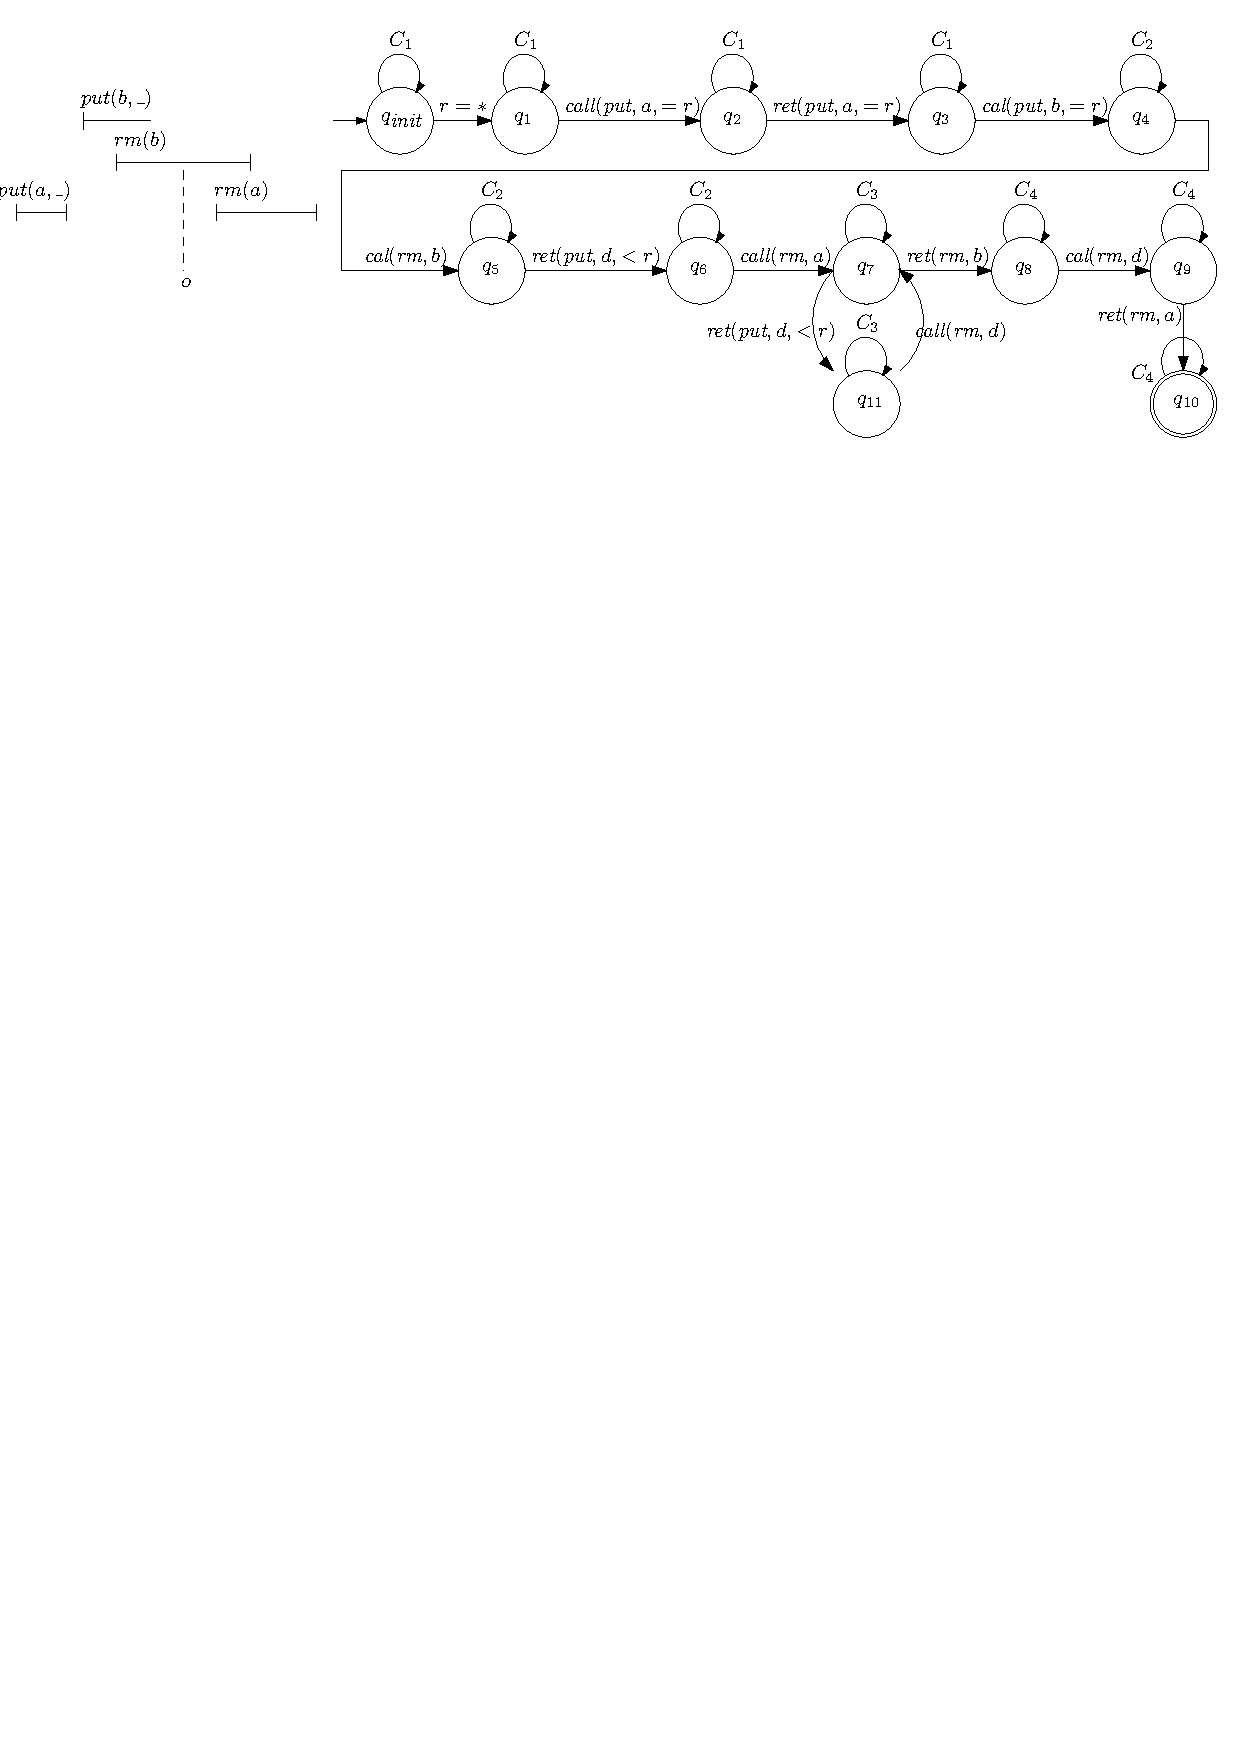
\includegraphics[width=0.8 \textwidth]{figures/PIC-Enumeration-WitnessAutomata.pdf}
%\vspace{-10pt}
  \caption{An enumerations and its register automaton}
  \label{fig:an enumeration and its witness automaton}
\end{figure}


\subsection{Reduce into State Reachability}
\label{subsec:combine step-by-step linearizability and co-regular}

We also prove that $\mathsf{UnmatchedMaxPriority}$ are co-regular in Appendix \ref{subsec:appendix co-regular of EPQ2Lar}, Appendix \ref{subsec:appendix co-regular of EPQ2Equal}, and prove that $\mathsf{EmptyRemove}$ are co-regular in Appendix \ref{subsec:co-regular of EPQ3}. Then we can see that $\seqPQ$ is co-regular.

\begin{restatable}{lemma}{EPQIsCoRegular}
\label{lemma:EPQ is co-regular}
$\seqPQ$ is co-regular.
\end{restatable}

By Lemma \ref{lemma:EPQ as multi in MRpri for history} and Lemma \ref{lemma:EPQ is co-regular}, we can finally reduce the verification of linearizability w.r.t $\seqPQ$ into a reachability problem, as illustrated by the following theorem, where $\textit{Auts}_{\textit{EPQ}}$ is the set of witness automata of this section.

\begin{restatable}{theorem}{ReduceEPQIntoStateReachability}
\label{lemma:reduce EPQ into state reachability}
Given a data-independence implementation $\mathcal{I}$. $\mathcal{I} \sqsubseteq \seqPQ$, if and only if, $\mathcal{I} \cap \textit{Auts}_{\textit{EPQ}} = \emptyset$.
\end{restatable}

When the data domain and priority domain are both fixed to be finite set, the register automata can be simulated with finite automata, and by Lemma \ref{lemma:reduce EPQ into state reachability}, checking linearizable w.r.t $\seqPQ$ is decidable.



